%!TEX root = thesis.tex
\section{Introduction}
\section{Lake-Analyzer}
\section{Foundtations}
	\subsection{Limniography}
	\subsection{Web Processing Service}
	\subsection{Streaming}
		\begin{itemize}
			\item
		\end{itemize}
		\subsubsection{WebSockets}
	\subsection{Matlab}
	\subsection{WPS4R}
	\subsection{Previous approaches}
	\begin{itemize}
		\item heavily format specific
		\item publishing results in a playlist that has to be checked constantly
		\item WPS splits inputs
	\end{itemize}
\section{Matlab WPS}
	\subsection{Configuration}
	\includecode[Matlab]
		{matlab-add-function.m}
		{\label{lst:matlab:example:fun}Matlab example function.}
	\includecode[YAML,morekeywords={function,connection,identifier,version,inputs,outputs,type}]
		{matlab-add-process-configuration.yaml}
		{\label{lst:matlab:example:yaml}Matlab process configuration describing the function in Listing \ref{lst:matlab:example:fun}.}
	\includecode[XML]
		{matlab-add-process-description.xml}
		{\label{lst:matlab:example:desc}Process description generated from the configuration in Listing \ref{lst:matlab:example:yaml}.}

	\subsection{Type Mapping}
	\begin{table}[!htb]
		\sffamily\centering
		\caption{\label{tab:matlab:typemapping}Type Mapping between Matlab and WPS Data}
		\begin{tabular}{@{}llcc@{}}
			\toprule
			&
			& \multicolumn{2}{b}{Matlab Type}\\
			\cmidrule(l){3-4}
			\multicolumn{1}{@{}b}{}
			& \multicolumn{1}{b}{Data}
			& \multicolumn{1}{b}{For single inputs}
			& \multicolumn{1}{b@{}}{For multiple inputs}\\
			\cmidrule(rl){2-2}
			\cmidrule(rl){3-3}
			\cmidrule(l){4-4}
			\textbf{Complex}      & \textit{any} & String  & Cell \\\midrule
			\textbf{Bounding Box} & -            & -       & -    \\\midrule
			\textbf{Literal}      & xs:int       & Numeric & Array\\
							      & xs:boolean   & Numeric & Array\\
							      & xs:dateTime  & Numeric & Array\\
							      & xs:double    & Numeric & Array\\
							      & xs:float     & Numeric & Array\\
							      & xs:byte      & Numeric & Array\\
							      & xs:short     & Numeric & Array\\
							      & xs:int       & Numeric & Array\\
							      & xs:long      & Numeric & Array\\
							      & xs:string    & String  & Cell \\
							      & xs:anyURI    & String  & Cell \\
			\bottomrule
		\end{tabular}
	\end{table}
	\subsection{Pooling}
	\subsection{License Issues}

	\begin{signedquote}{The MathWorks, Inc. Software License Agreement}
		4. LICENSE RESTRICTIONS.  The License is subject to the express restrictions
		set forth below. Licensee shall not, and shall not permit any Affiliate or any
		Third Party to:
			[...]
		    4.8. provide access (directly or indirectly) to the Programs via a web or
		    network Application, except as permitted in Article 8 of the Deployment
		    Addendum;
	\end{signedquote}

	\begin{signedquote}{The MathWorks, Inc. Software License Agreement - Deployment Addendum}
		8. WEB APPLICATIONS.  Licensee may not provide access to an entire Program
		or a substantial portion of a Program by means of a web interface.

		For the Network Concurrent User Activation Type.  Programs licensed under the
		Network Concurrent User Activation Type may be called via a web application,
		provided the web application does not provide access to the MATLAB command
		line, or any of the licensed Programs with code generation capabilities.  In
		addition, Licensed Users may not provide access to an entire Program or a
		substantial portion of a Program.  Such operation of an application via a web
		interface may be provided to an unlimited number of web browser clients, at no
		additional cost, for Licensee's own use for its Internal Operations, and for
		use by Third Parties.

		For the Network Named User and Standalone Named User Activation Types.
		Programs licensed under the Network Named User and Standalone Named User
		Activation Types may be called via a web application, provided the web
		application does not provide access to the MATLAB command line, or any of the
		licensed Programs with code generation capabilities, and such application is
		only accessed by designated Network Named User or Standalone Named User
		licensees of such Programs.

		Programs licensed under any other Activation Type may not be called via a web
		interface.
	\end{signedquote}
	\subsection{Implementation}
	\begin{figure}[!htb]
		\centering
		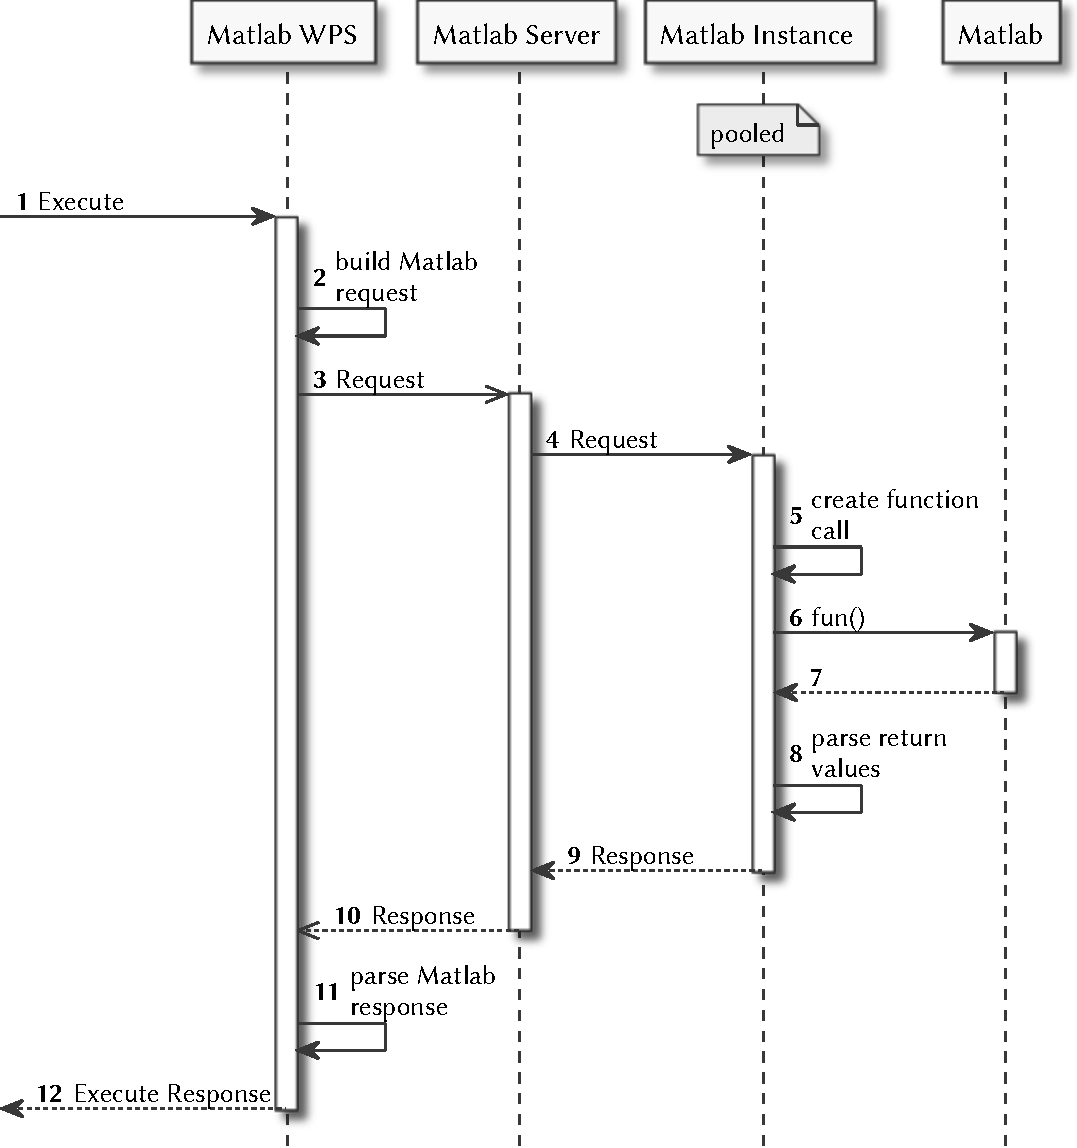
\includegraphics[width=.8\textwidth]{figures/sequence-diagramm-mwps.pdf}
		\caption{\label{fig:sd:mwps} Sequence diagram of the Matlab WPS.} %182x194
	\end{figure}
	\subsection{Lake-Analyzer WPS}
\section{Streaming WPS}
	\subsection{Input Types}\label{sec:streaming:input-types}
	\subsubsection{Static Inputs}
		\begin{itemize}
			\item see Listing \ref{lst:streaming:input:static}
			\item inputs common to every streaming iteration
			\item supplied when starting the streaming process
			\item merged with streaming inputs and forwarded to delegate
			\item configuration parameters, etc.
		\end{itemize}
		\includecode[XML]{streaming-input-static.xml}{\label{lst:streaming:input:static}Example for a Streaming WPS static inputs.}
	\subsubsection{Streaming Inputs}
		\begin{itemize}
			\item see Listing \ref{lst:streaming:input:streaming}
			\item provided for a single streaming iteration
			\item features all WPS input data types
		\end{itemize}
		\includecode[XML]{streaming-input-streaming.xml}{\label{lst:streaming:input:streaming}Example for a Streaming WPS streaming inputs.}
	\subsubsection{Reference Inputs}
		\begin{itemize}
			\item see Listing \ref{lst:streaming:input:reference}
			\item references the output of a previous or upcoming streaming iteration as an input for this iteration
			\item used to model dependencies between iterations/features/etc.
		\end{itemize}
		\includecode[XML]{streaming-input-reference.xml}{\label{lst:streaming:input:reference}Example for a Streaming WPS reference input.}
	\subsubsection{Polling inputs}
		\begin{itemize}
			\item Not implemented inside the streaming WPS.
			\item what to do if multiple polling inputs are defined?
			\item how to define polling frequency?
			\item how to define notifications?
			\item better handled on client side (see Figure \ref{fig:sd:polling})
		\end{itemize}
		\begin{figure}[!htb]
			\centering
			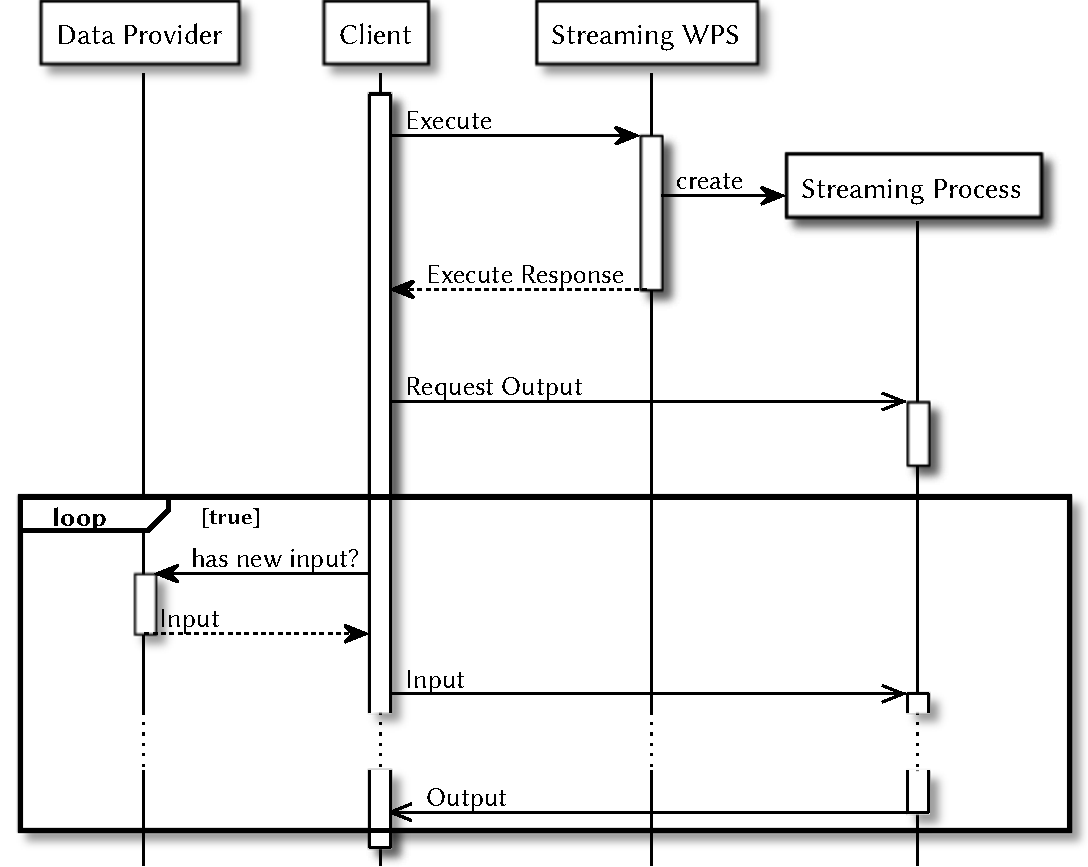
\includegraphics[width=.7868\textwidth]{figures/sequence-diagramm-polling.pdf}
			% 179x274
			\caption{\label{fig:sd:polling} Sequence diagram of the Streaming WPS.}
		\end{figure}

	\subsection{Dependencies}

	\begin{itemize}
		\item Directed acyclic graph $D=(V,E)$ with mutliple not interconnected subgraphs, probably quite sparse graphs.
		\item vertices are tasks, edges are dependencies to other tasks
		\item graph has to be acyclic as a cylce would produce a cyclic dependency that can not be resolved/executed
		\item see Figure \ref{fig:graph:unordered}
		\item topological ordering provides execution order see Figure \ref{fig:graph:ordered}
		\begin{itemize}
			\item ``A topological ordering, $ord_D$, of a directed acyclic graph $D = (V, E)$ maps each vertex to a priority value such that $ord_{D}(x) < ord_{D}(y)$ holds for all edges $x \rightarrow y \in E$.'' \citep{pearce2007dynamic}
			\item execution order = nodes sorted by descending $ord_D$
		 	\item linear time \citep{cormen2001introduction}: $\mathcal O(|V|+|E|)$  $\mathcal O(|E|)$ may vary between $\mathcal O(|V|)$ and  $O(|V|^2)$
		 \end{itemize}
		\item in contrast to e.g. package managers: non static graph, nodes and edges are added
		\item Recreating the topological ordering for every insertion can be costly \cite{pearce2007dynamic}
		\item \cite{pearce2007dynamic} provides dynamic algoritm for creating and maintaining the topological order, efficient on sparse graphs and constant factor slower on dense graphs
		\item graph only used to check for cyclic dependencies
		\item implementation listener based -> easier parallelization of execution
		\item streaming iterations are considered as tasks and can declare dependencies to other streaming iterations either by declaring mapping an input to the output of another streaming iteration (see Section \ref{sec:streaming:input-types}) or by declaring a explicit dependency on another streaming iteration
	\end{itemize}
	\begin{figure}[!htb]
		\centering
		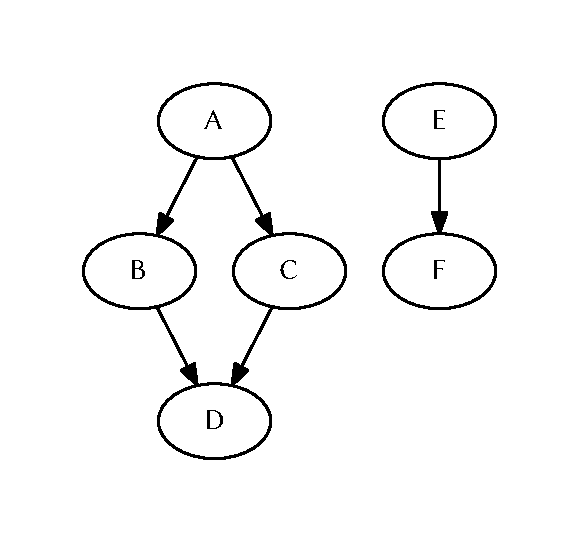
\includegraphics[width=.4474\textwidth]{figures/unordered-graph.pdf} % 98x92
		\caption{\label{fig:graph:unordered} Example for a dependency graph.}
	\end{figure}
	\begin{figure}[!htb]
		\centering
		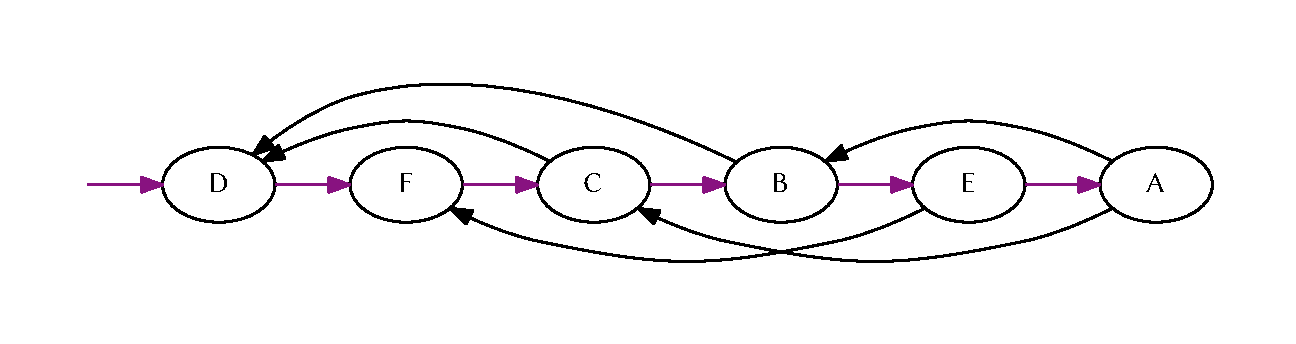
\includegraphics[width=1\textwidth]{figures/ordered-graph.pdf} % 219x58
		\caption{\label{fig:graph:ordered} Topological ordering for of the dependency graph in Figure \ref{fig:graph:unordered}.}
	\end{figure}

	\subsection{Protocoll}
	\subsection{Implementation}
	\begin{figure}[!htb]
		\centering
		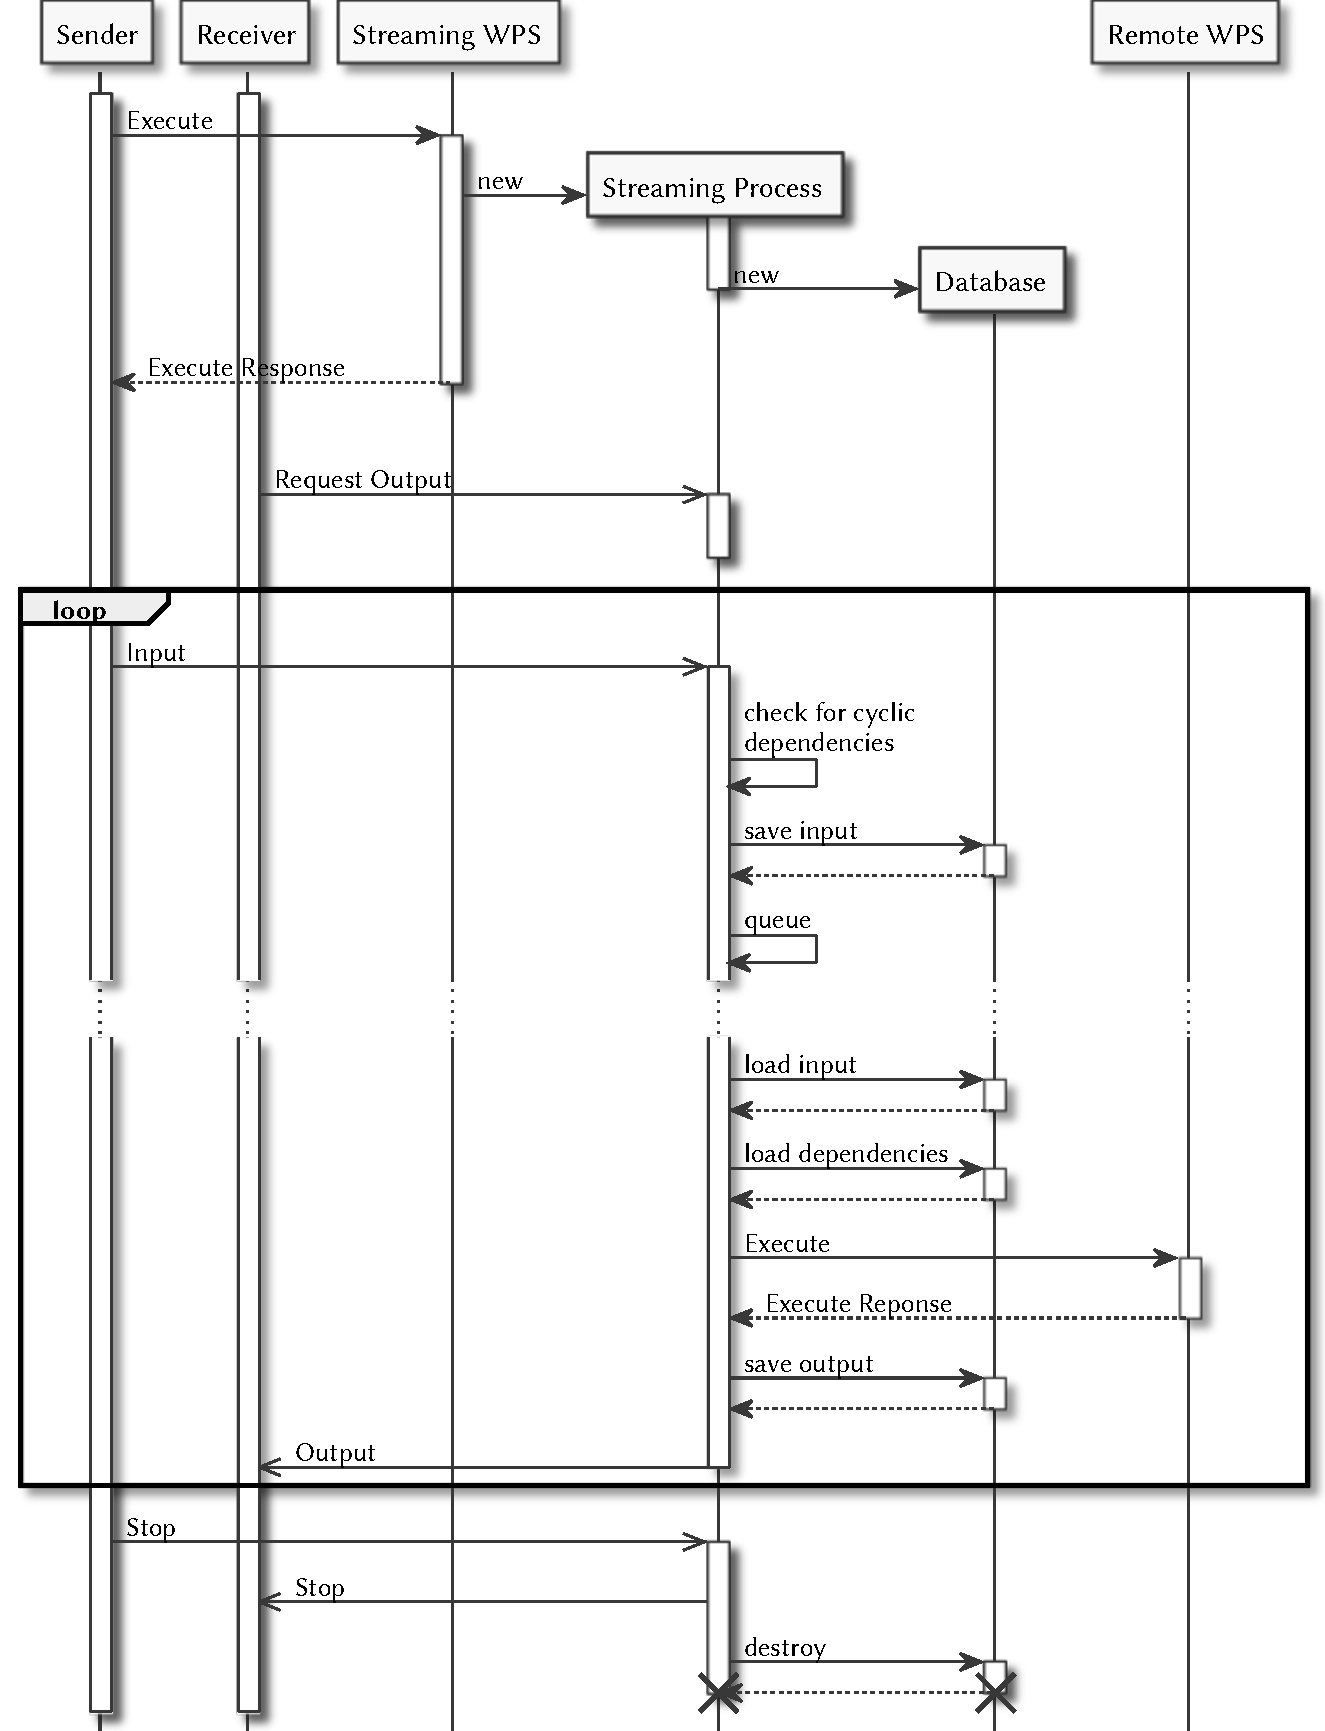
\includegraphics[width=.7868\textwidth]{figures/sequence-diagramm-swps.pdf}
		% 179x274
		\caption{\label{fig:sd:swps} Sequence diagram of the Streaming WPS.}
	\end{figure}
	\subsection{Client Implementation}
	\subsection{Streaming Lake-Analyzer WPS}
\section{Future Work}
\section{Conclusion}